\documentclass[11pt]{article}
\usepackage[utf8]{inputenc}
\usepackage{graphicx}
\usepackage{lineno}
\usepackage[a4paper, margin=2cm]{geometry}
\usepackage{titling}
\usepackage{setspace}

\renewcommand\maketitlehooka{\null\mbox{}\vfill}
\renewcommand\maketitlehookd{\vfill\null}

\title{Machine learning approaches to the evolution \\[0.5ex]and ecology of leaf shape\\[6cm]}
\author{Peter Zeng \\[5ex] Supervisor: \\[0.5ex]Will Pearse$^1$ Gemma Bramley$^2$ Alexander Zuntini$^2$\\[2ex]}
\date{%
    Supervisor Affiliation: \\[0.5ex]$^1$Department of Life Sciences(Silwood Park)\\%
    $^2$Kew Gardens\\[2ex] 
    Supervisor Contact Email:\\[0.5ex] Will Pearse: will.pearse@imperial.ac.uk \\[0.5ex] Gemma Bramley: g.bramley@kew.org \\[0.5ex] Alexander Zuntini: a.zuntini@kew.org\\[2ex]%
}



\begin{document}
\onehalfspacing 
\maketitle

\newpage

\begin{center}
\begin{Large} KeyWords: \end{Large} Machine Learning, Phylogeny, Leaf Shape, Quantification, Modelling, Classification
\\[9ex]
\end{center}


\section*{Introduction}
\linenumbers
Since people discover the potential of machine learning, different kinds of machine learning methods have been applied to scientific fields, which make it feasible to develop new algorithms or helps scientists save their time analyzing the data. Of these, the computer vision, an important part of machine learning, were widely used in the biological study \cite{jahne2000computer}. The automatic recognition of image based on features like shapes and patterns make it possible for people to use machine learning method to do the classification of images \cite{nanni2017handcrafted}. In this case, the image of plant's leaf can be ideal for the machine learning method to study \cite{fu2004machine}, as the leaf surface area, perimeter length and leaf compactness can be differ among different species. When people are studying the phylogeny of the plant, it will be effective to utilize machine learning methods to help people perform classification accurately and efficiently.
\\[3ex]
In the hope of helping develop new methods for studying the phylogeny of plant species, I will conduct a bioinformatics project based on machine learning methods. I will use the Angiosperm leaf's images, provided by the scientists in Kew Gardens, to quantify the morphology of the species. In this project, I will (1) update and extend an existing pipeline called "stalkless", which is aimed to record the individual leaf features \cite{pearse2018homogenization} (2) develop a machine learning pipeline, train it with the features of leaf, and perform classification (3) model the evolution of the estimated leaf shape using the phylogeny. 

\nolinenumbers
\section*{Methods and Materials}

\subsection*{1. Images of leaf}
\linenumbers
The angiosperm leaf images are collected by the scientists in Kew Gardens, which is related to the genera used in the BigTree, a part of the PAFTOL project held by the Kew Gardens \cite{baker2021comprehensive}. The PAFTOL project aims to equip people with the tools to accelerate efforts to document, identify and classify plants and fungi, explore their useful properties, understand their origins and evolution, and predict how species will respond to future environmental change.

\nolinenumbers
\subsection*{2. Update and extend the pipeline}
\linenumbers

I will update and extend an existing pipeline called "stalkless", a Python and R pipeline to record individual leaf surface area, perimeter length and leaf compactness, which is aimed to extract the morphology features of leaf images, and used for training the machine learning pipeline. The pipeline was used to quantify the leaf shape from herbarium specimens, and now I will try to apply it to the leaf images provided by scientists in Kew Gardens.

\nolinenumbers
\subsection*{3. Develop the machine learning pipeline}
\linenumbers

With the features provided by the stalkless pipeline, I will try to develop and train a machine learning model to perform the classification of these plant species. After training, the model should be accurate in classifying the plant species based on the features of their leaf shape.

\nolinenumbers
\subsection*{4. Model the evolution}
\linenumbers

I will be modelling the evolution of the estimated shape using the phylogeny. The phylogeny is provided from the Kew Garden

\nolinenumbers
\section*{Anticipated Outcomes}
\linenumbers

By the end of the project, I expect to (1) update and extend the "stalkless" pipeline, make it compatible with the plant images provided by Kew Gardens (2) develop a machine learning pipeline that can be used to classify the leaf image based on the morphology features of the leaf (3) model the evolution of the estimated leaf shape using the phylogeny. 

\nolinenumbers
\section*{Timeline}
\linenumbers

The scheduled timeline for the project is shown as Fig. 1:

\begin{figure}[h]
    \centering
    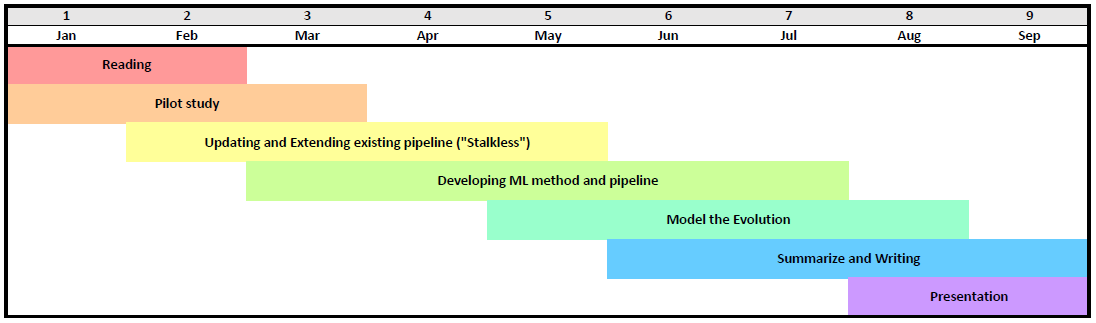
\includegraphics[width=1\textwidth]{Gantt_chart.png}
    \caption{Gantt chart of the project}
\end{figure}

\nolinenumbers
\section*{Budget}
\linenumbers

The project will need high performance computing for approximately 800 hours.

\nolinenumbers





\bibliographystyle{apalike}

  \bibliography{project_proposal.bib}

\newpage

\begin{center}
\begin{Large}I have seen and approved the proposal and the budget.\\[3ex]\end{Large}
\end{center}
\begin{Large}Supervisor Signature:\end{Large}
\\[3ex]
\begin{figure}[h]
\begin{flushright}
    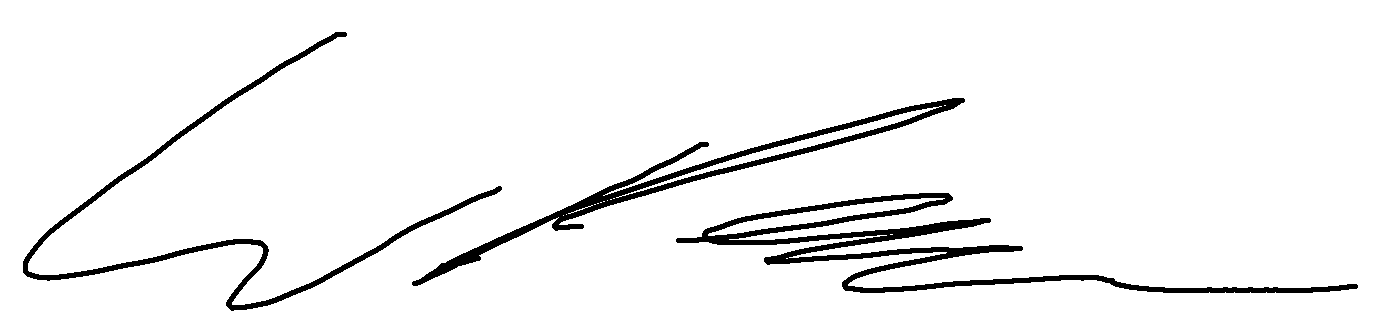
\includegraphics[width=0.4\textwidth]{will_pearse_signature.png}
    \end{flushright}
\end{figure}


\begin{flushright}
\begin{Large}Date: \end{Large}Dec 14 2021
    \end{flushright}




\end{document}
